\documentclass[11pt,letterpaper]{article}

% ============================================================================
% PACKAGES
% ============================================================================
\usepackage[utf8]{inputenc}
\usepackage[T1]{fontenc}
\usepackage{geometry}
\usepackage{graphicx}
\usepackage{xcolor}
\usepackage{tikz}
\usepackage{tcolorbox}
\usepackage{booktabs}
\usepackage{array}
\usepackage{longtable}
\usepackage{enumitem}
\usepackage{fancyhdr}
\usepackage{titlesec}
\usepackage{hyperref}
\usepackage{multirow}
\usepackage{tabularx}
\usepackage{float}
\usepackage{caption}
\usepackage{subcaption}
\usepackage{setspace}
\usepackage{parskip}

% ============================================================================
% PAGE LAYOUT
% ============================================================================
\geometry{
    left=1in,
    right=1in,
    top=1in,
    bottom=1in,
    headheight=20pt
}

% ============================================================================
% COLORS
% ============================================================================
\definecolor{primaryblue}{RGB}{0, 82, 147}
\definecolor{secondaryblue}{RGB}{52, 152, 219}
\definecolor{accentgreen}{RGB}{39, 174, 96}
\definecolor{warningorange}{RGB}{230, 126, 34}
\definecolor{lightgray}{RGB}{245, 245, 245}
\definecolor{darkgray}{RGB}{64, 64, 64}

% ============================================================================
% TIKZ LIBRARIES
% ============================================================================
\usetikzlibrary{shapes.geometric, arrows.meta, positioning, calc, fit, backgrounds}

% ============================================================================
% TCOLORBOX STYLES
% ============================================================================
\tcbuselibrary{skins, breakable}

\newtcolorbox{keyconceptbox}[1][]{
    colback=primaryblue!5,
    colframe=primaryblue,
    fonttitle=\bfseries,
    title=#1,
    breakable,
    enhanced,
    boxrule=1pt,
    left=8pt,
    right=8pt,
    top=6pt,
    bottom=6pt
}

\newtcolorbox{examplebox}[1][]{
    colback=accentgreen!5,
    colframe=accentgreen,
    fonttitle=\bfseries,
    title=#1,
    breakable,
    enhanced,
    boxrule=1pt,
    left=8pt,
    right=8pt,
    top=6pt,
    bottom=6pt
}

\newtcolorbox{notebox}[1][]{
    colback=warningorange!5,
    colframe=warningorange,
    fonttitle=\bfseries,
    title=#1,
    breakable,
    enhanced,
    boxrule=1pt,
    left=8pt,
    right=8pt,
    top=6pt,
    bottom=6pt
}

\newtcolorbox{summarybox}{
    colback=lightgray,
    colframe=darkgray,
    breakable,
    enhanced,
    boxrule=1pt,
    left=8pt,
    right=8pt,
    top=6pt,
    bottom=6pt
}

% ============================================================================
% HEADER AND FOOTER
% ============================================================================
\pagestyle{fancy}
\fancyhf{}
\fancyhead[L]{\textcolor{primaryblue}{\small Programs and Systems in Business Context}}
\fancyhead[R]{\textcolor{primaryblue}{\small Application Security Focus}}
\fancyfoot[C]{\thepage}
\renewcommand{\headrulewidth}{0.5pt}
\renewcommand{\headrule}{\hbox to\headwidth{\color{primaryblue}\leaders\hrule height \headrulewidth\hfill}}

% ============================================================================
% SECTION FORMATTING
% ============================================================================
\titleformat{\section}
    {\Large\bfseries\color{primaryblue}}
    {\thesection}{1em}{}
\titleformat{\subsection}
    {\large\bfseries\color{secondaryblue}}
    {\thesubsection}{1em}{}
\titleformat{\subsubsection}
    {\normalsize\bfseries\color{darkgray}}
    {\thesubsubsection}{1em}{}

% ============================================================================
% HYPERREF SETUP
% ============================================================================
\hypersetup{
    colorlinks=true,
    linkcolor=primaryblue,
    urlcolor=secondaryblue,
    citecolor=accentgreen
}

% ============================================================================
% DOCUMENT BEGINS
% ============================================================================
\begin{document}

% ============================================================================
% TITLE PAGE
% ============================================================================
\begin{titlepage}
    \centering
    \vspace*{1.5cm}
    
    {\Huge\bfseries\textcolor{primaryblue}{Programs and Systems\\in Business Context}\par}
    
    \vspace{0.75cm}
    
    {\LARGE\textcolor{secondaryblue}{A Comprehensive Guide with\\Application Security Focus}\par}
    
    \vspace{2cm}
    
    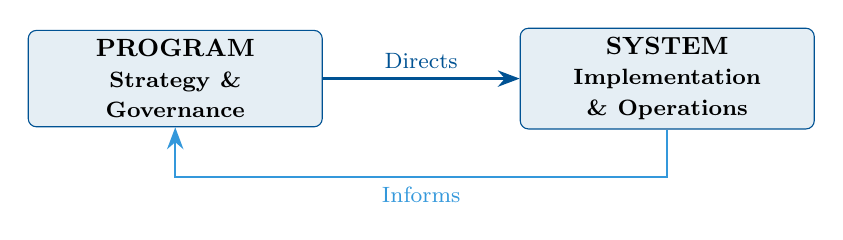
\begin{tikzpicture}[
        node distance=1.5cm,
        box/.style={rectangle, draw=primaryblue, fill=primaryblue!10, 
                    text width=3.5cm, minimum height=1.2cm, align=center,
                    rounded corners=3pt, font=\small\bfseries},
        arrow/.style={-{Stealth[scale=1.2]}, thick, primaryblue}
    ]
        \node[box] (program) {PROGRAM\\{\footnotesize Strategy \& Governance}};
        \node[box, right=2.5cm of program] (system) {SYSTEM\\{\footnotesize Implementation \& Operations}};
        
        \draw[arrow] (program.east) -- node[above, font=\footnotesize] {Directs} (system.west);
        \draw[arrow, secondaryblue] (system.south) -- ++(0,-0.6) -| node[below, pos=0.25, font=\footnotesize] {Informs} (program.south);
    \end{tikzpicture}
    
    \vspace{2.5cm}
    
    {\large\textcolor{darkgray}{Understanding the Strategic Relationship Between\\Organizational Programs and Implementation Systems}\par}
    
    \vfill
    
    {\large\today\par}
    
\end{titlepage}

% ============================================================================
% TABLE OF CONTENTS
% ============================================================================
\tableofcontents
\thispagestyle{empty}
\newpage
\setcounter{page}{1}

% ============================================================================
% EXECUTIVE SUMMARY
% ============================================================================
\section{Executive Summary}

In the complex landscape of modern business operations, understanding the distinction and relationship between \textbf{programs} and \textbf{systems} is fundamental to organizational success. This document provides a comprehensive exploration of these concepts, using application security as a primary illustrative example.

\begin{summarybox}
\textbf{Core Distinction:} A \textit{program} is the structured strategic initiative that defines goals, policies, and scope, while a \textit{system} is the collection of tools, processes, infrastructure, and people that implements that program in day-to-day operations.
\end{summarybox}

This relationship can be understood through a simple analogy: the program is the \textit{blueprint}, and the system is the \textit{building} constructed from that blueprint. Without a well-defined program, systems lack direction and coherence. Without robust systems, programs remain theoretical exercises with no practical impact.

The document examines how programs define the ``what'' and ``why'' of organizational initiatives, while systems address the ``how.'' Using application security as a case study, we explore how these concepts manifest across the software development lifecycle, from design and development through production operations and governance.

Key topics covered include program governance frameworks, system implementation strategies, technology selection, process integration, organizational alignment, and practical approaches to identifying gaps between strategic intent and operational capability.

% ============================================================================
% SECTION 1: INTRODUCTION
% ============================================================================
\section{Introduction to Programs and Systems}

\subsection{Foundational Concepts}

Modern organizations operate through interconnected programs and systems that translate strategic vision into operational reality. Understanding these foundational concepts is essential for leaders, architects, and practitioners across all business domains.

\subsubsection{Defining ``Program'' in Business Context}

A \textbf{program} is a structured, long-term initiative designed to achieve specific organizational objectives. Programs are characterized by their strategic nature, defined scope, and governance frameworks. They establish the boundaries within which operational activities occur and provide the rationale for resource allocation and decision-making.

Programs answer fundamental questions about organizational direction:

\begin{itemize}[leftmargin=2em]
    \item What objectives are we pursuing?
    \item Why are these objectives important to the organization?
    \item What constraints and standards govern our approach?
    \item How do we measure success and progress?
    \item Who has authority and accountability?
\end{itemize}

\subsubsection{Defining ``System'' in Business Context}

A \textbf{system} is the collection of tangible and intangible elements that operationalizes a program. Systems encompass technologies, processes, people, and policies working together to achieve program objectives. They represent the practical machinery of implementation.

Systems address operational questions:

\begin{itemize}[leftmargin=2em]
    \item How do we accomplish program objectives?
    \item What tools and technologies support our work?
    \item What processes guide daily activities?
    \item Who performs specific functions and how are they organized?
    \item How do we monitor, measure, and improve operations?
\end{itemize}

\subsection{The Relationship Between Programs and Systems}

The relationship between programs and systems is symbiotic and dynamic. Programs provide direction and governance; systems provide capability and execution. Neither can succeed in isolation.

\begin{figure}[H]
\centering
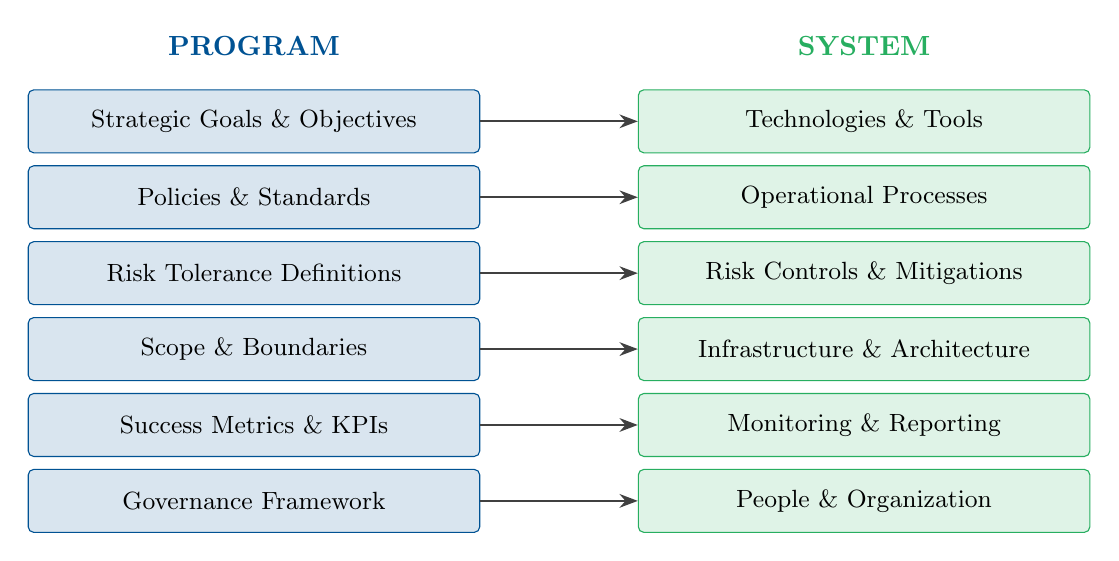
\begin{tikzpicture}[
    node distance=0.8cm,
    every node/.style={font=\small},
    programbox/.style={rectangle, draw=primaryblue, fill=primaryblue!15, 
                       text width=5.5cm, minimum height=0.8cm, align=center,
                       rounded corners=2pt},
    systembox/.style={rectangle, draw=accentgreen, fill=accentgreen!15, 
                      text width=5.5cm, minimum height=0.8cm, align=center,
                      rounded corners=2pt},
    titlebox/.style={rectangle, draw=none, fill=none, 
                     text width=5.5cm, align=center, font=\bfseries}
]
    % Program side
    \node[titlebox, text=primaryblue] (ptitle) {PROGRAM};
    \node[programbox, below=0.3cm of ptitle] (p1) {Strategic Goals \& Objectives};
    \node[programbox, below=0.15cm of p1] (p2) {Policies \& Standards};
    \node[programbox, below=0.15cm of p2] (p3) {Risk Tolerance Definitions};
    \node[programbox, below=0.15cm of p3] (p4) {Scope \& Boundaries};
    \node[programbox, below=0.15cm of p4] (p5) {Success Metrics \& KPIs};
    \node[programbox, below=0.15cm of p5] (p6) {Governance Framework};
    
    % System side
    \node[titlebox, text=accentgreen, right=2cm of ptitle] (stitle) {SYSTEM};
    \node[systembox, below=0.3cm of stitle] (s1) {Technologies \& Tools};
    \node[systembox, below=0.15cm of s1] (s2) {Operational Processes};
    \node[systembox, below=0.15cm of s2] (s3) {Risk Controls \& Mitigations};
    \node[systembox, below=0.15cm of s3] (s4) {Infrastructure \& Architecture};
    \node[systembox, below=0.15cm of s4] (s5) {Monitoring \& Reporting};
    \node[systembox, below=0.15cm of s5] (s6) {People \& Organization};
    
    % Connecting arrows
    \draw[-{Stealth}, thick, darkgray] (p1.east) -- (s1.west);
    \draw[-{Stealth}, thick, darkgray] (p2.east) -- (s2.west);
    \draw[-{Stealth}, thick, darkgray] (p3.east) -- (s3.west);
    \draw[-{Stealth}, thick, darkgray] (p4.east) -- (s4.west);
    \draw[-{Stealth}, thick, darkgray] (p5.east) -- (s5.west);
    \draw[-{Stealth}, thick, darkgray] (p6.east) -- (s6.west);
\end{tikzpicture}
\caption{Mapping Program Elements to System Components}
\label{fig:program-system-mapping}
\end{figure}

\begin{keyconceptbox}[Key Insight]
The program is the blueprint and governance layer that sets direction and rules. The system is the concrete machine---the engines, gears, and dashboards---that actually carries them out across the organizational lifecycle.
\end{keyconceptbox}

% ============================================================================
% SECTION 2: THE PROGRAM
% ============================================================================
\section{The Program: Strategy and Governance}

\subsection{Program as the ``What and Why''}

A program defines the strategic intent behind organizational initiatives. It establishes what the organization seeks to protect, achieve, or transform, and articulates the rationale for these pursuits. Programs provide the intellectual and governance foundation upon which systems are built.

\subsubsection{Core Components of a Program}

Every well-structured program contains several essential components that guide its implementation and evolution:

\begin{table}[H]
\centering
\renewcommand{\arraystretch}{1.3}
\begin{tabularx}{\textwidth}{>{\bfseries}l X}
\toprule
\textbf{Component} & \textbf{Description} \\
\midrule
Vision \& Mission & The aspirational end-state and the program's fundamental purpose \\
Objectives & Specific, measurable goals the program seeks to achieve \\
Scope Definition & Clear boundaries identifying what is included and excluded \\
Policy Framework & Governing rules, standards, and compliance requirements \\
Risk Tolerance & Acceptable levels of risk across different categories \\
Success Criteria & Metrics and indicators used to evaluate program effectiveness \\
Governance Model & Decision-making authority, escalation paths, and accountability \\
Resource Allocation & Budget, personnel, and infrastructure commitments \\
\bottomrule
\end{tabularx}
\caption{Core Components of an Organizational Program}
\label{tab:program-components}
\end{table}

\subsubsection{Strategic Questions Addressed by Programs}

Programs answer foundational strategic questions that shape all downstream activities:

\paragraph{What Are We Protecting or Achieving?} Programs define the assets, capabilities, or outcomes that require attention. In application security, this includes customer data, intellectual property, system availability, and regulatory compliance.

\paragraph{Why Is This Important?} Programs articulate the business rationale, connecting initiatives to organizational mission, competitive advantage, regulatory requirements, or stakeholder expectations.

\paragraph{What Standards Do We Follow?} Programs establish the frameworks, methodologies, and compliance requirements that govern operations. These may include industry standards (OWASP, NIST, ISO), regulatory requirements (GDPR, PCI-DSS, HIPAA), or internal policies.

\paragraph{What Is Our Risk Tolerance?} Programs define acceptable risk levels across different categories, enabling informed decision-making about resource allocation and control implementation.

\subsection{Program Governance Framework}

Effective programs require robust governance structures that ensure accountability, enable decision-making, and provide oversight mechanisms.

\subsubsection{Governance Hierarchy}

\begin{figure}[H]
\centering
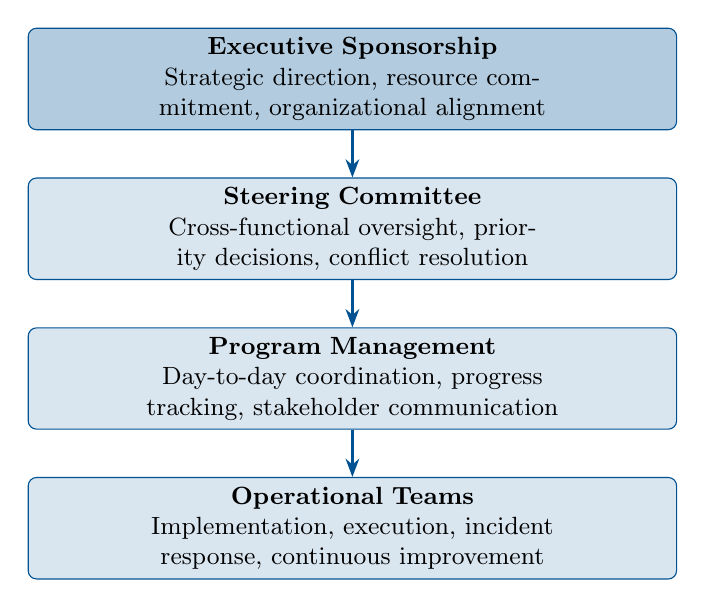
\begin{tikzpicture}[
    node distance=0.6cm,
    level/.style={rectangle, draw=primaryblue, fill=primaryblue!15, 
                  text width=8cm, minimum height=1cm, align=center,
                  rounded corners=3pt, font=\small}
]
    \node[level, fill=primaryblue!30] (exec) {\textbf{Executive Sponsorship}\\Strategic direction, resource commitment, organizational alignment};
    \node[level, below=of exec] (steer) {\textbf{Steering Committee}\\Cross-functional oversight, priority decisions, conflict resolution};
    \node[level, below=of steer] (mgmt) {\textbf{Program Management}\\Day-to-day coordination, progress tracking, stakeholder communication};
    \node[level, below=of mgmt] (ops) {\textbf{Operational Teams}\\Implementation, execution, incident response, continuous improvement};
    
    \draw[-{Stealth}, thick, primaryblue] (exec.south) -- (steer.north);
    \draw[-{Stealth}, thick, primaryblue] (steer.south) -- (mgmt.north);
    \draw[-{Stealth}, thick, primaryblue] (mgmt.south) -- (ops.north);
\end{tikzpicture}
\caption{Program Governance Hierarchy}
\label{fig:governance-hierarchy}
\end{figure}

\subsubsection{Key Governance Functions}

\begin{itemize}[leftmargin=2em]
    \item \textbf{Policy Development:} Creating, maintaining, and communicating program policies that establish expectations and requirements.
    \item \textbf{Resource Management:} Allocating budget, personnel, and infrastructure to support program objectives.
    \item \textbf{Performance Monitoring:} Tracking metrics and indicators to assess program effectiveness and identify improvement opportunities.
    \item \textbf{Risk Oversight:} Monitoring risk exposure, reviewing risk assessments, and approving risk treatment decisions.
    \item \textbf{Compliance Assurance:} Ensuring adherence to regulatory requirements and internal standards.
    \item \textbf{Continuous Improvement:} Identifying lessons learned and driving program maturation.
\end{itemize}

% ============================================================================
% SECTION 3: THE SYSTEM
% ============================================================================
\section{The System: Implementation and Operations}

\subsection{System as the ``How''}

While programs define strategic intent, systems provide the operational capability to realize that intent. A system is the comprehensive collection of technologies, processes, people, and infrastructure that transforms program objectives into daily activities and measurable outcomes.

\subsection{Core System Components}

\subsubsection{Technologies and Tools}

Technologies form the technical backbone of any system. In the context of application security, these include:

\begin{table}[H]
\centering
\renewcommand{\arraystretch}{1.3}
\begin{tabularx}{\textwidth}{>{\bfseries}l l X}
\toprule
\textbf{Category} & \textbf{Technology} & \textbf{Purpose} \\
\midrule
Code Analysis & SAST & Static analysis of source code to identify vulnerabilities \\
Runtime Testing & DAST & Dynamic testing of running applications for security flaws \\
Composition Analysis & SCA & Identification of vulnerabilities in third-party dependencies \\
Runtime Protection & RASP & Real-time application protection and attack prevention \\
Perimeter Defense & WAF & Web application firewall for traffic filtering \\
Posture Management & ASPM & Unified visibility and risk management across applications \\
Secret Detection & Secret Scanning & Prevention of credential and key exposure in code \\
Container Security & CSPM/CWPP & Cloud and container workload protection \\
\bottomrule
\end{tabularx}
\caption{Application Security Technology Categories}
\label{tab:security-technologies}
\end{table}

\subsubsection{Processes and Workflows}

Processes define how work is accomplished within the system. Effective security systems incorporate processes throughout the software lifecycle:

\begin{examplebox}[Key Security Processes]
\begin{itemize}[leftmargin=1.5em, itemsep=0.2em]
    \item Threat modeling during design phases
    \item Secure code review workflows integrated into pull requests
    \item Automated security gates in CI/CD pipelines
    \item Vulnerability triage and prioritization processes
    \item Patch management and remediation tracking
    \item Security testing in QA environments
    \item Incident response and breach management
    \item Security training and awareness programs
\end{itemize}
\end{examplebox}

\subsubsection{People and Organization}

Human capital is essential to system effectiveness. The organizational dimension includes:

\begin{itemize}[leftmargin=2em]
    \item \textbf{Dedicated Security Teams:} Application security engineers, penetration testers, security architects
    \item \textbf{Embedded Security Champions:} Developers with security expertise distributed across engineering teams
    \item \textbf{Leadership:} Security managers, CISOs, and executives with security oversight responsibilities
    \item \textbf{Extended Team:} DevOps engineers, SREs, and operations staff with security responsibilities
\end{itemize}

\subsubsection{Policies and Standards}

Operational policies translate program-level requirements into actionable guidance:

\begin{itemize}[leftmargin=2em]
    \item Secure coding standards and guidelines
    \item Access control and authorization policies
    \item Data classification and handling requirements
    \item Third-party and vendor security requirements
    \item Exception and waiver processes
    \item Audit and compliance procedures
\end{itemize}

\subsection{System Integration Points}

Systems do not operate in isolation. Effective security systems integrate with broader organizational systems and workflows:

\begin{figure}[H]
\centering
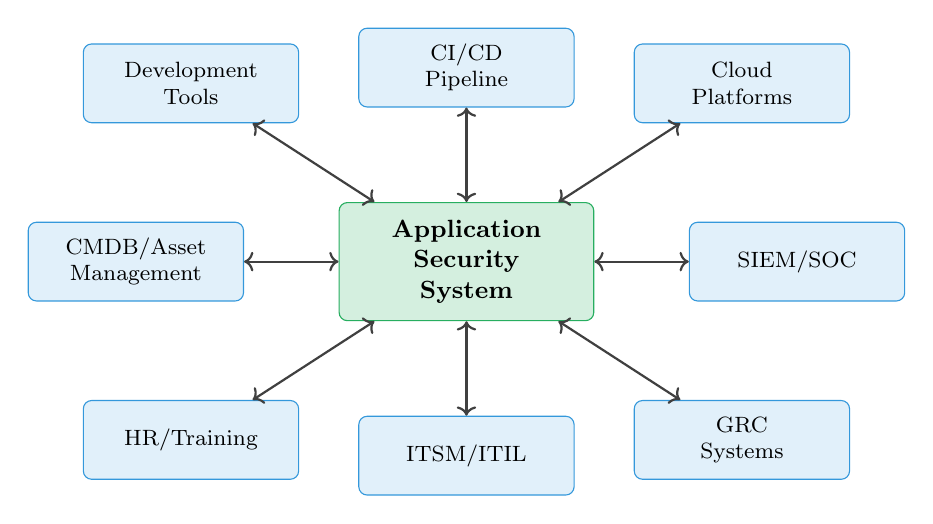
\begin{tikzpicture}[
    node distance=1cm,
    mainbox/.style={rectangle, draw=accentgreen, fill=accentgreen!20, 
                    text width=3cm, minimum height=1.5cm, align=center,
                    rounded corners=3pt, font=\small\bfseries},
    extbox/.style={rectangle, draw=secondaryblue, fill=secondaryblue!15, 
                   text width=2.5cm, minimum height=1cm, align=center,
                   rounded corners=3pt, font=\footnotesize}
]
    \node[mainbox] (core) {Application\\Security\\System};
    
    \node[extbox, above left=1cm and 0.5cm of core] (dev) {Development\\Tools};
    \node[extbox, above=1.2cm of core] (cicd) {CI/CD\\Pipeline};
    \node[extbox, above right=1cm and 0.5cm of core] (cloud) {Cloud\\Platforms};
    \node[extbox, right=1.2cm of core] (siem) {SIEM/SOC};
    \node[extbox, below right=1cm and 0.5cm of core] (grc) {GRC\\Systems};
    \node[extbox, below=1.2cm of core] (itil) {ITSM/ITIL};
    \node[extbox, below left=1cm and 0.5cm of core] (hr) {HR/Training};
    \node[extbox, left=1.2cm of core] (cmdb) {CMDB/Asset\\Management};
    
    \foreach \ext in {dev, cicd, cloud, siem, grc, itil, hr, cmdb}
        \draw[thick, darkgray, <->] (core) -- (\ext);
\end{tikzpicture}
\caption{Security System Integration Points}
\label{fig:integration-points}
\end{figure}

% ============================================================================
% SECTION 4: APPLICATION SECURITY CASE STUDY
% ============================================================================
\section{Application Security: A Comprehensive Case Study}

\subsection{Program Definition}

An application security program is a strategic initiative designed to protect software assets throughout their lifecycle. It establishes the governance framework, policies, and objectives that guide all security activities related to application development and operation.

\subsubsection{Program Goal Statement}

\begin{keyconceptbox}[Application Security Program Goal]
Reduce the risk of data breaches, operational disruptions, and reputational damage caused by application vulnerabilities through systematic security practices integrated into every stage of the software development lifecycle.
\end{keyconceptbox}

\subsubsection{Program Policy Examples}

Well-defined programs establish clear, measurable policies:

\begin{table}[H]
\centering
\renewcommand{\arraystretch}{1.3}
\begin{tabularx}{\textwidth}{>{\bfseries}p{3cm} X}
\toprule
\textbf{Policy Area} & \textbf{Example Policy Statement} \\
\midrule
Standards Compliance & All internet-facing applications must meet OWASP Application Security Verification Standard (ASVS) Level 2 or higher. \\
Remediation SLAs & Critical vulnerabilities must be remediated within 7 days; High within 30 days; Medium within 90 days. \\
SDLC Integration & Security activities must be embedded into every phase of the software development lifecycle. \\
Testing Requirements & All applications must undergo SAST, DAST, and SCA testing before production deployment. \\
Third-Party Risk & All third-party components must be evaluated for known vulnerabilities before integration. \\
Training & All developers must complete secure coding training annually. \\
\bottomrule
\end{tabularx}
\caption{Example Application Security Program Policies}
\label{tab:security-policies}
\end{table}

\subsection{System Implementation Across the SDLC}

The application security system implements program objectives through activities and technologies aligned with each phase of the software development lifecycle.

\begin{figure}[H]
\centering
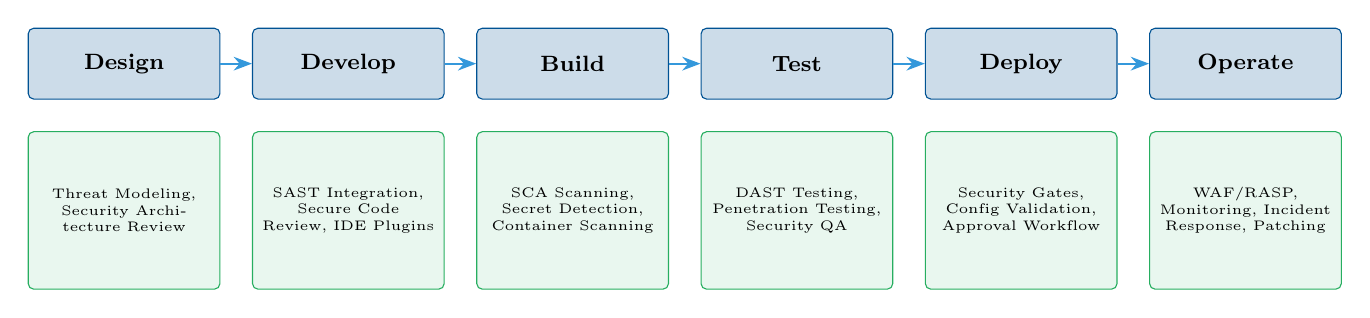
\begin{tikzpicture}[
    node distance=0.3cm,
    phase/.style={rectangle, draw=primaryblue, fill=primaryblue!20, 
                  text width=2.2cm, minimum height=0.9cm, align=center,
                  rounded corners=2pt, font=\footnotesize\bfseries},
    activity/.style={rectangle, draw=accentgreen, fill=accentgreen!10, 
                     text width=2.2cm, minimum height=2cm, align=center,
                     rounded corners=2pt, font=\tiny}
]
    % Phases
    \node[phase] (p1) {Design};
    \node[phase, right=0.4cm of p1] (p2) {Develop};
    \node[phase, right=0.4cm of p2] (p3) {Build};
    \node[phase, right=0.4cm of p3] (p4) {Test};
    \node[phase, right=0.4cm of p4] (p5) {Deploy};
    \node[phase, right=0.4cm of p5] (p6) {Operate};
    
    % Activities
    \node[activity, below=0.4cm of p1] (a1) {Threat Modeling, Security Architecture Review};
    \node[activity, below=0.4cm of p2] (a2) {SAST Integration, Secure Code Review, IDE Plugins};
    \node[activity, below=0.4cm of p3] (a3) {SCA Scanning, Secret Detection, Container Scanning};
    \node[activity, below=0.4cm of p4] (a4) {DAST Testing, Penetration Testing, Security QA};
    \node[activity, below=0.4cm of p5] (a5) {Security Gates, Config Validation, Approval Workflow};
    \node[activity, below=0.4cm of p6] (a6) {WAF/RASP, Monitoring, Incident Response, Patching};
    
    % Arrows
    \draw[-{Stealth}, thick, secondaryblue] (p1) -- (p2);
    \draw[-{Stealth}, thick, secondaryblue] (p2) -- (p3);
    \draw[-{Stealth}, thick, secondaryblue] (p3) -- (p4);
    \draw[-{Stealth}, thick, secondaryblue] (p4) -- (p5);
    \draw[-{Stealth}, thick, secondaryblue] (p5) -- (p6);
\end{tikzpicture}
\caption{Security Activities Across the Software Development Lifecycle}
\label{fig:sdlc-security}
\end{figure}

\subsubsection{Design and Development Phase}

During design and development, the security system focuses on proactive vulnerability prevention:

\paragraph{Threat Modeling:} Systematic analysis of application architecture to identify potential threats, attack vectors, and required controls. Threat models inform security requirements and design decisions before code is written.

\paragraph{SAST Integration:} Static Application Security Testing tools integrated into development environments and CI pipelines scan source code for security vulnerabilities during development. Early detection reduces remediation cost and timeline.

\paragraph{Secure Code Review:} Peer review processes with security-focused checklists ensure that code changes are evaluated for common vulnerability patterns before merge.

\subsubsection{Testing and Pre-Production Phase}

Testing phases validate security controls and identify vulnerabilities before production exposure:

\paragraph{DAST Execution:} Dynamic Application Security Testing against staging environments identifies runtime vulnerabilities that static analysis cannot detect, including authentication flaws, session management issues, and injection vulnerabilities.

\paragraph{Security Test Plans:} Formalized security testing procedures integrated into QA processes ensure consistent coverage and documentation of security validation activities.

\paragraph{Penetration Testing:} Expert-led adversarial testing simulates real-world attacks to validate control effectiveness and identify complex vulnerability chains.

\subsubsection{Production Phase}

Production systems require active protection and continuous monitoring:

\paragraph{WAF Deployment:} Web Application Firewalls filter malicious traffic and provide virtual patching capabilities for applications that cannot be immediately remediated.

\paragraph{RASP Implementation:} Runtime Application Self-Protection agents monitor application behavior and block attacks in real-time without requiring external infrastructure.

\paragraph{Incident Response:} Documented runbooks and on-call processes ensure rapid, effective response to security incidents affecting production applications.

\paragraph{Vulnerability Management:} Continuous processes for tracking, prioritizing, and remediating vulnerabilities across the application portfolio.

\subsection{Governance and Visibility}

\subsubsection{Application Security Posture Management}

An Application Security Posture Management (ASPM) platform serves as the central nervous system of the security program, providing unified visibility across all applications, environments, and security activities.

\begin{notebox}[ASPM Capabilities]
ASPM platforms aggregate data from multiple security tools to provide:
\begin{itemize}[leftmargin=1.5em, itemsep=0.15em]
    \item Consolidated vulnerability inventory across all applications
    \item Risk scoring and prioritization based on business context
    \item Coverage analysis to identify security testing gaps
    \item Trend analysis and program health metrics
    \item Compliance reporting and audit support
    \item Integration with ticketing and workflow systems
\end{itemize}
\end{notebox}

\subsubsection{Metrics and Reporting}

Effective governance requires clear metrics that demonstrate program effectiveness:

\begin{table}[H]
\centering
\renewcommand{\arraystretch}{1.3}
\begin{tabularx}{\textwidth}{>{\bfseries}p{3.5cm} X p{3cm}}
\toprule
\textbf{Metric Category} & \textbf{Example Metrics} & \textbf{Purpose} \\
\midrule
Vulnerability Metrics & Mean time to remediate (MTTR), vulnerability age distribution, open vulnerability count & Measure remediation effectiveness \\
Coverage Metrics & Percentage of applications with SAST/DAST, threat model coverage, training completion rates & Assess program reach \\
Risk Metrics & Risk score trends, critical finding counts, exploited vulnerability tracking & Quantify security posture \\
Process Metrics & Security gate pass rates, false positive rates, finding recurrence rates & Evaluate process efficiency \\
\bottomrule
\end{tabularx}
\caption{Application Security Program Metrics}
\label{tab:security-metrics}
\end{table}

% ============================================================================
% SECTION 5: PRACTICAL IMPLEMENTATION
% ============================================================================
\section{Practical Implementation Guidance}

\subsection{Gap Analysis: Program vs. System Alignment}

Organizations should periodically assess alignment between program requirements and system capabilities. This gap analysis identifies areas where systems fail to implement program objectives or where program policies are unrealistic given current capabilities.

\subsubsection{Gap Analysis Framework}

\begin{table}[H]
\centering
\renewcommand{\arraystretch}{1.3}
\begin{tabularx}{\textwidth}{>{\bfseries}p{3cm} X X}
\toprule
\textbf{Program Requirement} & \textbf{System Capability} & \textbf{Gap Identification} \\
\midrule
SAST on all code & SAST deployed for 60\% of repos & 40\% coverage gap \\
Critical vuln SLA: 7 days & Average MTTR: 21 days & Process/resource gap \\
Annual pen testing & Last pen test: 18 months ago & Scheduling/budget gap \\
Developer training & 45\% completion rate & Adoption/enforcement gap \\
Third-party risk review & Manual, inconsistent process & Tooling/automation gap \\
\bottomrule
\end{tabularx}
\caption{Example Gap Analysis Results}
\label{tab:gap-analysis}
\end{table}

\subsection{Maturity Model Considerations}

Programs and systems evolve through maturity stages. Understanding current maturity helps organizations prioritize improvements and set realistic expectations.

\begin{figure}[H]
\centering
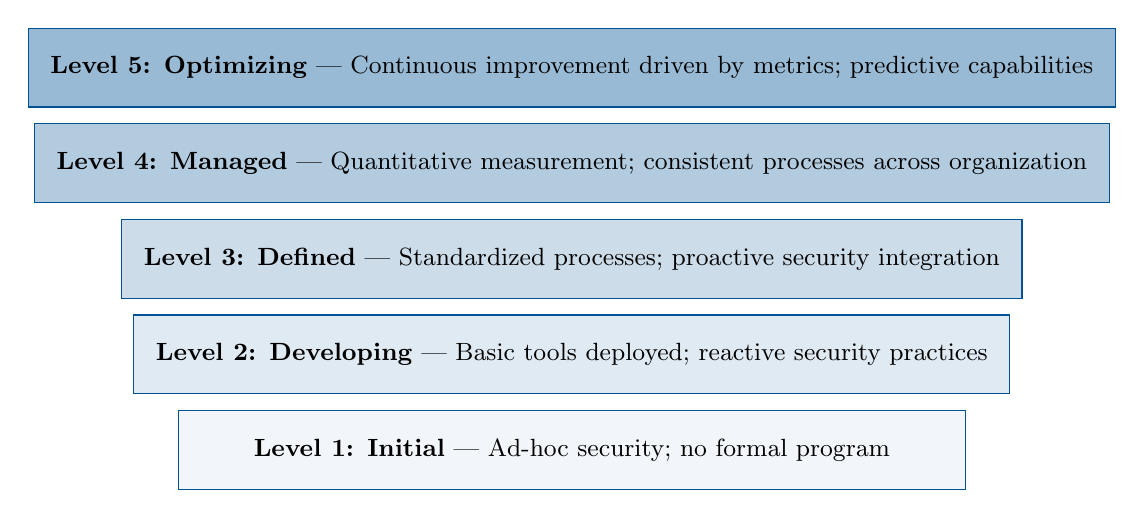
\begin{tikzpicture}[
    node distance=0.2cm,
    level/.style={rectangle, draw=primaryblue, minimum width=10cm, minimum height=1cm, 
                  align=left, font=\small, inner sep=8pt}
]
    \node[level, fill=primaryblue!40] (l5) {\textbf{Level 5: Optimizing} --- Continuous improvement driven by metrics; predictive capabilities};
    \node[level, fill=primaryblue!30, below=of l5] (l4) {\textbf{Level 4: Managed} --- Quantitative measurement; consistent processes across organization};
    \node[level, fill=primaryblue!20, below=of l4] (l3) {\textbf{Level 3: Defined} --- Standardized processes; proactive security integration};
    \node[level, fill=primaryblue!12, below=of l3] (l2) {\textbf{Level 2: Developing} --- Basic tools deployed; reactive security practices};
    \node[level, fill=primaryblue!5, below=of l2] (l1) {\textbf{Level 1: Initial} --- Ad-hoc security; no formal program};
\end{tikzpicture}
\caption{Security Program Maturity Model}
\label{fig:maturity-model}
\end{figure}

\subsection{Common Implementation Challenges}

\subsubsection{Program-Level Challenges}

\begin{itemize}[leftmargin=2em]
    \item Lack of executive sponsorship and organizational commitment
    \item Unclear or conflicting priorities between security and delivery velocity
    \item Insufficient budget allocation for security tooling and personnel
    \item Policies that are unrealistic given current organizational capabilities
    \item Poor communication of program objectives across stakeholder groups
\end{itemize}

\subsubsection{System-Level Challenges}

\begin{itemize}[leftmargin=2em]
    \item Tool sprawl creating alert fatigue and integration complexity
    \item High false positive rates undermining developer trust
    \item Insufficient integration between security tools and development workflows
    \item Skills gaps in security engineering and operations
    \item Legacy applications resistant to modern security practices
\end{itemize}

\subsection{Success Factors}

Organizations that successfully align programs and systems typically exhibit these characteristics:

\begin{examplebox}[Critical Success Factors]
\begin{enumerate}[leftmargin=1.5em, itemsep=0.3em]
    \item \textbf{Executive Commitment:} Visible leadership support and resource allocation
    \item \textbf{Clear Accountability:} Defined ownership for program and system components
    \item \textbf{Developer Experience:} Security tools integrated into existing workflows with minimal friction
    \item \textbf{Measurable Objectives:} Specific, trackable metrics tied to business outcomes
    \item \textbf{Continuous Feedback:} Regular assessment and adjustment based on operational data
    \item \textbf{Risk-Based Prioritization:} Focus on highest-impact activities given limited resources
    \item \textbf{Cultural Integration:} Security viewed as shared responsibility, not external constraint
\end{enumerate}
\end{examplebox}

% ============================================================================
% SECTION 6: CONCLUSION
% ============================================================================
\section{Conclusion}

The relationship between programs and systems is fundamental to organizational effectiveness across all domains. Programs provide the strategic direction, governance framework, and policy structure that define what an organization seeks to achieve and why. Systems provide the operational machinery---the tools, processes, people, and infrastructure---that translates program objectives into daily activities and measurable outcomes.

\begin{summarybox}
\textbf{Key Takeaways:}

\textbf{1. Complementary Roles:} Programs and systems are interdependent. Programs without systems remain theoretical; systems without programs lack direction and coherence.

\textbf{2. The Program Defines ``What and Why'':} Programs establish goals, policies, scope, risk tolerance, and governance structures that guide all downstream activities.

\textbf{3. The System Defines ``How'':} Systems implement program objectives through technologies, processes, people, and operational policies.

\textbf{4. Continuous Alignment:} Regular gap analysis ensures that systems effectively implement program requirements and that programs remain realistic given system capabilities.

\textbf{5. Maturity Evolution:} Both programs and systems evolve through maturity stages, requiring ongoing investment and improvement.
\end{summarybox}

In the context of application security, this framework provides a clear model for understanding how strategic security objectives translate into operational security practices. The program establishes requirements like vulnerability remediation timelines, testing coverage expectations, and compliance standards. The system implements these requirements through SAST/DAST tools, CI/CD integration, security teams, and governance platforms like ASPM.

Organizations that clearly distinguish between program and system responsibilities, maintain alignment between them, and invest in both strategic governance and operational capability are best positioned to achieve their security objectives while supporting business agility.

\vspace{1cm}

\begin{center}
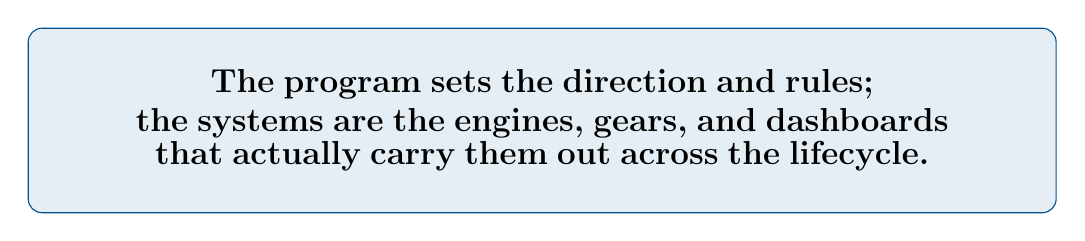
\begin{tikzpicture}
    \node[draw=primaryblue, fill=primaryblue!10, rounded corners=5pt, 
          text width=12cm, align=center, inner sep=15pt] {
        \textbf{\large The program sets the direction and rules;\\the systems are the engines, gears, and dashboards\\that actually carry them out across the lifecycle.}
    };
\end{tikzpicture}
\end{center}

% ============================================================================
% APPENDIX
% ============================================================================
\newpage
\appendix
\section{Appendix: Tool Categories Reference}

\begin{longtable}{>{\bfseries}p{2.5cm} p{4cm} p{6.5cm}}
\toprule
\textbf{Acronym} & \textbf{Full Name} & \textbf{Description} \\
\midrule
\endfirsthead
\toprule
\textbf{Acronym} & \textbf{Full Name} & \textbf{Description} \\
\midrule
\endhead
\bottomrule
\endfoot
SAST & Static Application Security Testing & Analyzes source code or binaries for security vulnerabilities without executing the application \\
DAST & Dynamic Application Security Testing & Tests running applications by simulating attacks to identify runtime vulnerabilities \\
SCA & Software Composition Analysis & Identifies vulnerabilities and license issues in third-party and open-source components \\
IAST & Interactive Application Security Testing & Combines SAST and DAST approaches using agents within running applications \\
RASP & Runtime Application Self-Protection & Provides real-time protection by monitoring and blocking attacks from within the application \\
WAF & Web Application Firewall & Filters and monitors HTTP traffic to protect web applications from common attacks \\
ASPM & Application Security Posture Management & Provides unified visibility and risk management across the application security program \\
CSPM & Cloud Security Posture Management & Monitors cloud infrastructure for security misconfigurations and compliance violations \\
CWPP & Cloud Workload Protection Platform & Protects cloud workloads including containers, VMs, and serverless functions \\
SBOM & Software Bill of Materials & Inventory of all components and dependencies in a software application \\
SDLC & Software Development Lifecycle & Framework defining phases of software development from planning to maintenance \\
CI/CD & Continuous Integration / Continuous Deployment & Automated processes for building, testing, and deploying software changes \\
\end{longtable}

\section{Appendix: Further Reading}

The following resources provide additional depth on application security programs and systems:

\begin{itemize}[leftmargin=2em]
    \item OWASP Application Security Verification Standard (ASVS)
    \item NIST Secure Software Development Framework (SSDF)
    \item BSIMM (Building Security In Maturity Model)
    \item OWASP Software Assurance Maturity Model (SAMM)
    \item ISO/IEC 27034 Application Security Standards
    \item CIS Software Supply Chain Security Guide
\end{itemize}

\end{document}
